\documentclass{IEEEtran}

\usepackage{mathtools}
\usepackage{graphicx}
\usepackage{subfig}
\usepackage{verbatim}
\usepackage{algpseudocode}
\usepackage{natbib}
\usepackage{url}
\usepackage{listings}
\usepackage[spanish]{babel}
\usepackage[utf8x]{inputenc}
\usepackage{float}


\begin{document}

\title{Informe Tarea No 1}
\date {Marzo de 2013}
\author{\IEEEauthorblockN{Tatiana Lopez Guevara \\}
\IEEEauthorblockA{Universidad Tecnológica de Pereira\\
zepolitat@utp.edu.co }}
\maketitle


\begin{abstract}
El presente documento explica los resultados obtenidos al aplicar
y remover una distorción proyectiva sobre un conjunto de imágenes.
El objetivo principal era aplicar las técnicas vistas
en la primera parte del curso de Computer Vision para afianzar 
los conceptos aprendidos.
\end{abstract}

\begin{IEEEkeywords}
Computer Vision
\end{IEEEkeywords}

\section{Introducción}
\IEEEPARstart{P}{ara} el desarrollo del proyecto se construyeron
los siguientes archivos fuente:

\begin{itemize}
\item \textbf{zpart1.m} ~\\
Archivo principal de la parte 1 de la tarea.
Contiene los parámetros (ruta de la imágen y coordenadas de los 8 puntos)
así como las invoaciones a las funciones que en su conjunto, remueven
la distroción de la imágen.

\item \textbf{zimread.m} ~\\
Carga una imágen y retorna su representación como un vector 2D de
$W*H$ filas y 3 columnas de color. Por la agilidad de su operación,
esta representación es la usada principalmente para realizar 
las operaciones sobre la imágen.
Adicionalmente, retorna una matrix tridimensional 
de $H$ filas, $W$ columnas y 3 canales de color RGB principalmente
para el despliegue en pantalla.

\item \textbf{zfindH.m} ~\\
Encuentra una homografía $H$ a partir de las 2 parejas de 4
puntos aplicando (\ref{eq:h}).

\item \textbf{transformCorner.m} ~\\
Calcula las esquinas de una imágen dado el ancho y el alto
y aplica una homografía sobre estas. Esta función invoca a transformX.

\item \textbf{transformImg.m} ~\\
Genera la combinación de puntos $(x,y)$ de una imágen y aplica
una homografía invocando a transformX.m.

\item \textbf{transformX.m} ~\\
Aplica una homografía a una matrix de puntos de la forma
$[x_1 x_2 .. x_N; y_1 y_2 .. y_N]$ y la normaliza.

\item \textbf{bilineal.m} ~\\
Realiza una interpolación bilineal de una imágen en representación
vectorial de tamaño $[(W*H) , 3]$ y de un conjunto de índices, posiblemente
de valores no enteros, que la referencian.

\item \textbf{zpart2.m} ~\\
Archivo principal de la parte 2 de la tarea.
Contiene los parámetros (ruta de las imágenes y coordenadas de los 8 puntos)
así como las invoaciones a las funciones que en su conjuno, sobrepone
una imágen planar sobre otra que tiene alguna distorción.

\end{itemize} 

Las homografías $H$ usadas, corresponden al grupo de trasnformaciones
PL(3) de 8 $DoF$ y por lo tanto requiere de 8 puntos para caracterizarla
\cite{hartley2000multiple}

\section{Primera Parte}

El objetivo de la primera parte era remover la distorción de una imágen tomada con
una cámara aplicando interpolación bilineal.

Se tomaron las siguientes convenciones en el código fuente:
\begin{itemize}
\item La imágen distorcionada se toma como el conjunto de
puntos sobre los que existe una distorción $x^{'}$
y todo lo relacionado con éstas tiene el prefijo la letra $i$
(inicial).
\item La imágen que será creada al remover la distorción
representa el conjunto de puntos $x$ y la información
relacionada con éstos tiene como prefijo la letra $f$
(final).
\end{itemize} 

Los parámetros de la imágen y de las coordenadas de los
4 puntos en la imágen inicial y sus 4 puntos equivalentes
en la imágen final se ingresan en las primeras líneas del
script $zpart1.m$ .

\begin{lstlisting}[frame=single]
[iVecImg, iImg, iW, iH] = 
    zimread('../imgs/scan.jpg');

xp=[32  354 528 138];
yp=[204 138 568 677];
x =[100 460 460 100];
y =[150 150 670 670];

imshow(iImg);
hold on; 
scatter(xp,yp,5,'r');
\end{lstlisting}
%\lstinputlisting{snippets/zpart1_1.m}[frame=single]

El archivo $scan.jpg$ representa la imagen distorcionada
de la figura \ref{fig:p1iImg}.

\begin{figure}%[H]
\caption{Imágen Inicial}
\centering

\includegraphics[width=6cm,natwidth=401,natheight=652]{imgs/p1iImg.png}
\label{fig:p1iImg}
\end{figure} 

Al insertar estos 4 puntos $x$ y sus equivalentes $x^{'}$
en \ref{eq:h}, se hallaron los parámetros 
de la matriz de proyección $H$.

\begin{equation}
  \begin{pmatrix}
    h_{11} \\ h_{12} \\ h_{13}\\ h_{21} \\ h_{22} \\ h_{23}\\
    h_{31} \\ h_{32} \\ h_{33}\\
 \end{pmatrix}
 =
 \begin{pmatrix}
  x_1 & y_1 & 0 & 0 & 0 & -x_1^{'} x_1 & -x_1^{'} y_1 \\
  0 & 0 & 0 & x_1 & y_1 & -y_1^{'} x_1 & -y_1^{'} y_1 \\
    &   &   &     &  \vdots & & &  \\
  x_4 & y_4 & 0 & 0 & 0 & -x_4^{'} x_4 & -x_4^{'} y_4 \\
  0 & 0 & 0 & x_4 & y_4 & -y_4^{'} x_4 & -y_4^{'} y_4 \\
 \end{pmatrix}^{-1}
 \begin{pmatrix}
    x^{'}_1 \\ y^{'}_1 \\ \vdots \\ x^{'}_4 \\ y^{'}_4 \\
 \end{pmatrix}
\label{eq:h}
\end{equation} 

Lo primero que se hizo fue hallar el tamaño de la imágen 
final. Para esto se aplicó la homografía inversa sobre
las esquinas de la imágen cargada empleando (\ref{eq:x}).

\begin{equation}
x=H^{-1} x^{'}
\label{eq:x}
\end{equation} 

En este punto, existían 2 opciones para remover la 
distorción:
 
\begin{enumerate}
\item Partir de la imágen inicial, calculando para cada
uno de sus puntos $(x^{'},y^{'})$ el correspondiente valor
de $(x,y)$ usando (\ref{eq:x}) . 
\item Partir de la imágen final, calculando para cada
uno de sus puntos $(x,y)$ el correspondiente valor
de $(x^{'},y^{'})$ mediante (\ref{eq:xp}) . 
\end{enumerate} 

La primera opción, aunque parece más natural, tiene el inconveniente
de que no necesariamente se asigna un valor para todos los pixeles de
la imágen final, dejando espacios vacíos (de color negro) que se debe
rellenar en un paso posterior. 
A pesar de que se ensayaron las 2 opciones, sólo se dejó la segunda
en el código y es la que se continuará explicando.

Teniendo entonces el tamaño de la imágen, se procedió a 
encontrar para cada punto $(x,y)$ de la imágen
final, su equivalente $(x^{'},y^{'})$  con el fin de conocer 
el color RGB del pixel correspondiente a $(x,y)$. Cabe notar
que a pesar de que (\ref{eq:xp}) hace referencia a la transformación 
de un solo punto, en el desarrollo se usó la representación matricial
en donde $x$ es el conjunto de puntos de la forma 
$[x_1 y_1 1; x_2 y_2 1; .. x_N y_N 1]'$ y por lo tanto $x'$ contiene
todos los puntos transformados de $x$;


\begin{equation}
x^{'}=H x
\label{eq:xp}
\end{equation} 

Sin embargo, los puntos $(x^{'},y^{'})$ que se obtienen de 
(\ref{eq:xp}) pueden no ser enteros y por lo tanto
se aplicó la técnica de interpolación bilineal (\ref{eq:ibilineal})
\cite{BilinearWiki}.

\begin{align}
f(x,y) \approx \frac{1}{(x_2 - x_1)(y_2 - y_1)}(
&f(Q_{11})(x_2-x)(y_2-y)+\nonumber\\
&f(Q_{21})(x-x_1)(y_2-y)+\nonumber\\
&f(Q_{12})(x_2-x)(y-y_1)+\nonumber\\
&f(Q_{22})(x-x_1)(y-y_1))
\label{eq:ibilineal}
\end{align} 

Donde para este caso la distancia entre las coordenadas de las cuales se
obtendrá el promedio ponderado de un punto desconocido es 1, con lo que 
el término del denominador se vuelve 1.

Finalmente, al aplicar la homografía y la interpolación bilineal sobre
la figura \ref{fig:p1iImg} se obtubo la figura \ref{fig:p1fImg}.

\begin{figure}%[H]
\caption{Imágen Final}
\centering
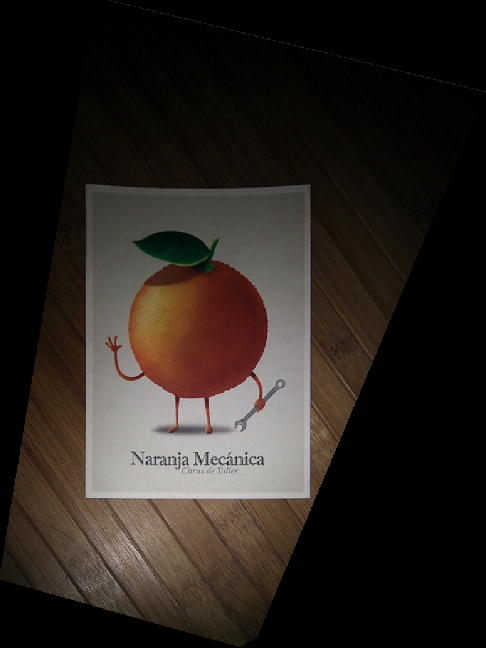
\includegraphics[width=6cm,natwidth=486,natheight=648]{imgs/p1fImg.png}
\label{fig:p1fImg}
\end{figure} 

\section{Segunda Parte}

La segunda parte del proyecto consistió en utilizar la misma técnica 
para aumentar una escena, sobreponiendo una imagen planar sobre 
una imagen base, con la perspectiva correcta.

La imágen planar usada en el proyecto corresponde a la mostrada en la figura
\ref{fig:p2Planar}. El objetivo entonces era aplicar una distorción
proyectiva sobre ésta con el fin de sobreponera en los puntos marcados
con rojo de la figura \ref{fig:p2iImg}.
\begin{figure}[H]
\caption{Imágen Planar}
\centering

\includegraphics[width=3cm,natwidth=500,natheight=753]{imgs/domokun.jpg}
\label{fig:p2Planar}
\end{figure} 

\begin{figure}[H]
\caption{Imágen con distorción proyectiva}
\centering
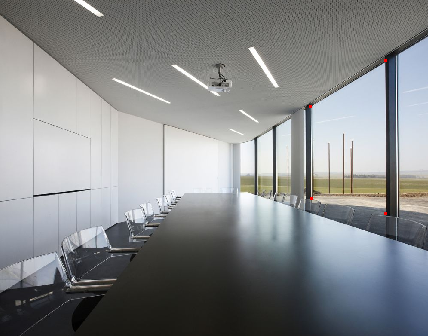
\includegraphics[width=7cm,natwidth=428,natheight=336]{imgs/p2iImg.png}
\label{fig:p2iImg}
\end{figure} 

De forma similar a la parte 1, se realizó el cálculo de la matrix de 
transformación $H$ a partir de los 8 puntos dados. Luego, ésta se usó
para aplicar la distorción proyetiva sobre cada punto de la imágen planar 
mediante (\ref{eq:xp}) .
El resultado obtenido se puede ver en la figura \ref{fig:p2fImg}.

\begin{figure}[H]
\caption{Imágen planar sobrepuesta en imágen con distorción proyectiva}
\centering
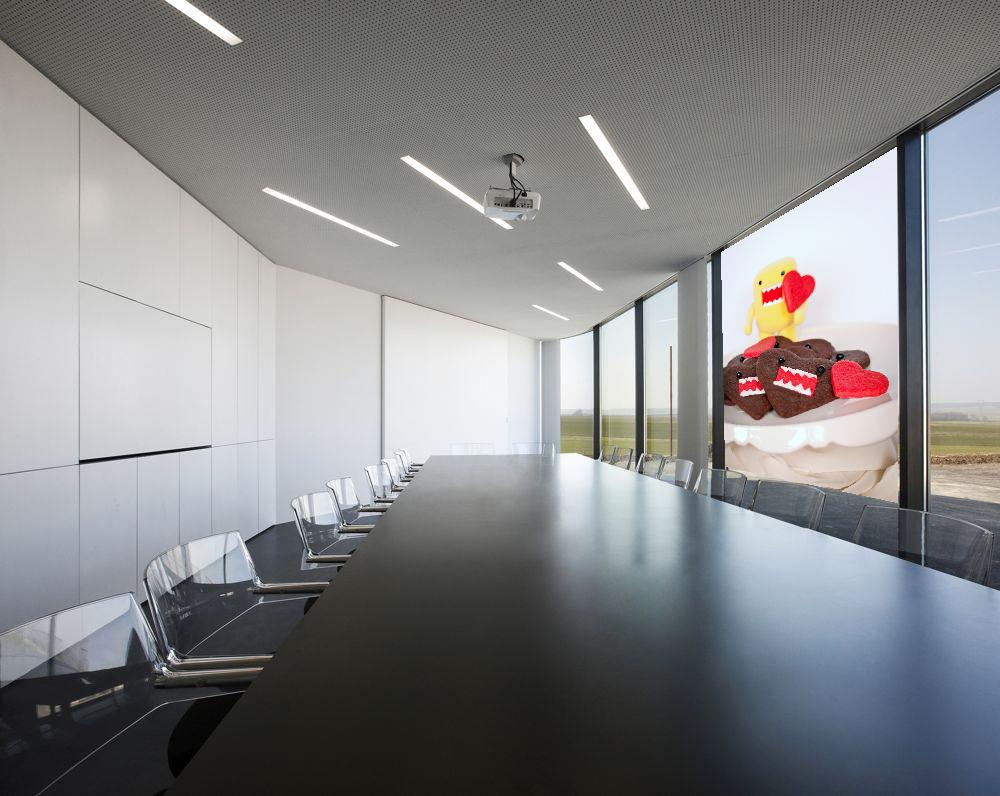
\includegraphics[width=7cm,natwidth=1000,natheight=796]{imgs/p2fImg.jpg}
\label{fig:p2fImg}
\end{figure} 

\section{Conclusiones}
\begin{itemize}
\item Al no tener limitaciones de las posibles transformaciones que
tenía la imágen origen, se debía asumir que éstas podían tener
elementos de rotación, traslación y escalamiento. Por lo tanto, 
las homografías $H$ con las que se debía trabajar pertenecen al grupo
PL(3) de 8 $DoF$ requiriendo 8 puntos para encontrarla.

\item Existen dos posibilidades de remover la distorción proyectiva
de una imágen. La primera es partir de la imágen inicial, calculando para cada
uno de sus puntos el valor equivalente en la imágen destino. La segunda
es el proceso inverso partiendo de cada pixel de la imágen destino hacia la
inicial.

\item La interpolación bilineal permite realizar una aproximación suave de un
pixel no entero a partir de sus pixeles vecinos, mientras que aproximar directamente
a un entero, hace que la imágen se vea más pixelada ya que es una aproximación "dura".
\end{itemize} 

\bibliographystyle{plain}
\bibliography{biblio}

\end{document}
